% Author: Paul Shao
% Email: paulshaoyuqiao1@berkeley.edu
Suppose that you are the engineer tasked with the job of making Google Maps. For this, you want to be able to determine the position of a user using satellite information. In particular, assume that you know $d_1, d_2$ and $d_3$, the distances from the user's cellphone to 3 satellites. You know the positions of these satellites to be $\vec{a_1}, \vec{a_2}$, and $\vec{a_3}$. Here's a simplified figure demonstrating what's been given so far:

\begin{figure}[H]
    \centering
    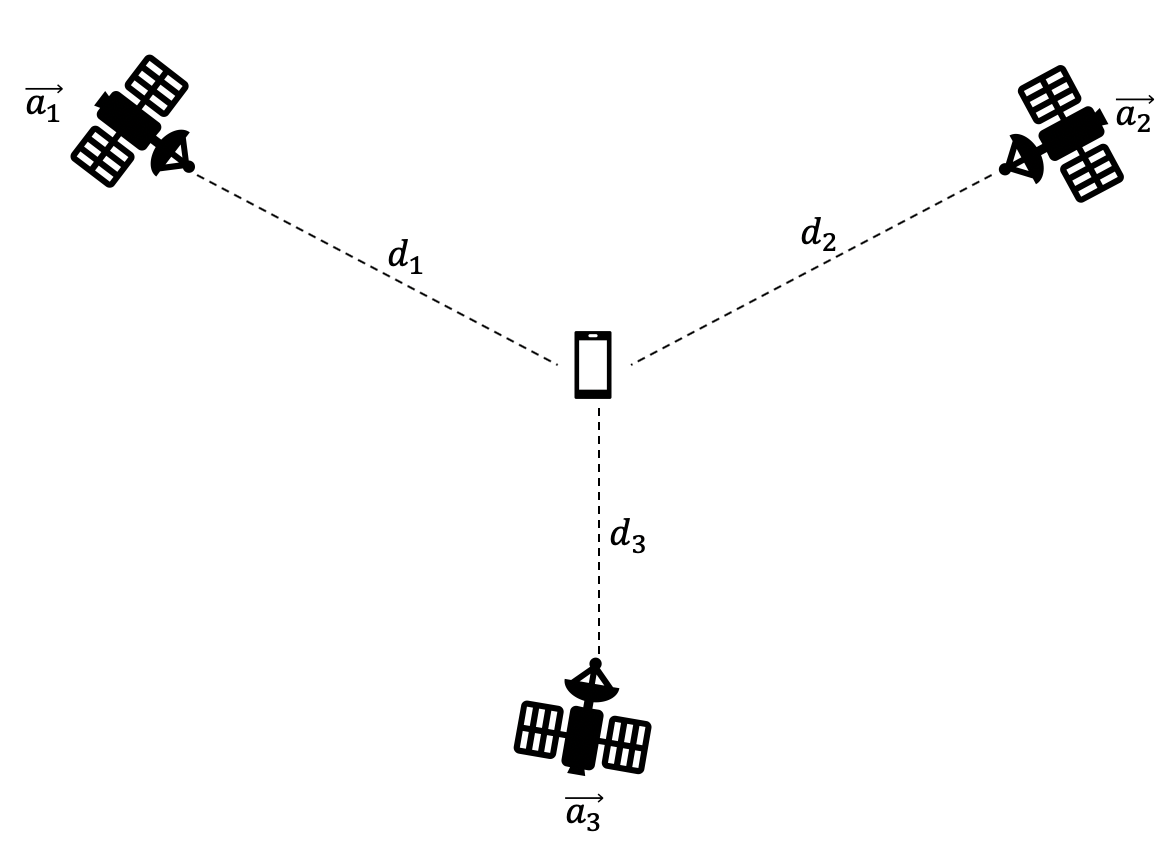
\includegraphics[scale=0.5]{../trilateration.png}
\end{figure}

\textit{Note: What does it mean when we say "position"? You can assume that these positions are taken relative to some common origin. Say, the Google HQ - Mountain View, CA.}

\begin{enumerate}
\item{Suppose the user's location (or the phone's location) is given by the vector $\vec{x}$, write out a system of equations representing the distances from the user to all 3 satellites (Express your answer in terms of $\vec{x}, \vec{a_1}, \vec{a_2}, \vec{a_3}, d_1, d_2, $ and $d_3$).}

\note{
    Be sure to encourage the students to utilize the provided figure and consider the problem geometrically. In addition, also remind the students that the norm of a vector $\|\vec{v}\|$ represents the length of the vector and motivate them to first find the vectors that can represent the path between each satellite and the user.
}

\sol{
$$\| \vec{x} - \vec{a_1} \| = d_1$$
$$\| \vec{x} - \vec{a_2} \| = d_2$$
$$\| \vec{x} - \vec{a_3} \| = d_3$$
These equations relate the position of the user to the distance between the user and each satellite.
}

\item{Rewrite these equations in terms of inner products of vectors. Are these equations linear with respect to $\vec{x}$?}

\note{
    Be sure to explain to students what it means for an expression to be \textbf{linear with respect to $\vec{x}$}: it means that we can write the expression as a \textbf{linear (max degree = 1) combination of the individual entries in $\vec{x}$}. Motivate them with some non-linear examples such as for an $n$-dimensional vector $\vec{x}$, $\vec{x}^T \vec{x}$:
    $$\vec{x}^T \vec{x} = \|x\|^2 = x_1^2 +x_2^2 + \dots + x_n^2.$$
    Here, we can see that the expression contains quadratic (or non-linear) terms of the entries in $\vec{x}$. \\ \\
    \textbf{In addition, explain to the students what the intuition behind squaring both sides of the equations is.} Since the left sides of all three equations are vector norms, squaring the norms will give us the inner products of these vectors with themselves. This comes from the property:
    $$\|\vec{x}\|^2 = \left \langle \vec{x}, \vec{x} \right \rangle = \vec{x}^T \vec{x}.$$
}

\sol{
By squaring each side, we get the following:
$$(\vec{x} - \vec{a_1})^T(\vec{x} - \vec{a_1}) = d_1^2$$
$$(\vec{x} - \vec{a_2})^T(\vec{x} - \vec{a_2}) = d_2^2$$
$$(\vec{x} - \vec{a_3})^T(\vec{x} - \vec{a_3}) = d_3^2$$

Then, expanding the LHS, we get:
$$\vec{x}^T\vec{x} - 2\vec{a_1}^T\vec{x} + \vec{a_1}^T\vec{a_1} = d_1^2$$
$$\vec{x}^T\vec{x} - 2\vec{a_2}^T\vec{x} + \vec{a_2}^T\vec{a_2} = d_2^2$$
$$\vec{x}^T\vec{x} - 2\vec{a_3}^T\vec{x} + \vec{a_3}^T\vec{a_3} = d_3^2$$

These equations are not linear in $\vec{x}$, because they contain an $\vec{x}^T\vec{x}$ term.
}

\item{
Are there any non-linear terms in the equations from the previous part? Using \textbf{elimination of variables}, rewrite everything as a system of \textbf{linear} equations.
}

\note{
It is likely that some students will realize throughout the process that to cancel out the non-linear terms, they have to subtract equations from each other, which consequently reduces the total number of usable (distinct) equations. Be sure to explain to them that the reason we will have less "usable" equations is because as we are subtracting equations from each other, we are "equvalently" creating linear combinations of these expressions, and if we still maintain the same number of equations, one of them in the end can be \textbf{written as a linear combination of the other two} (implies linear dependence!). That means the third equation we have \textbf{won't contribute any new information}, since it can be derived from the previous two.
}

\sol{
The non-linear terms in the equations are $\vec{x}^T \vec{x}$, but we can use variable elimination to get rid of them.

Subtract the first equation from the other 2 in order to eliminate the $\vec{x}^T\vec{x}$ term. We get the following:
$$2(\vec{a_1}^T\vec{x} - \vec{a_2}^T\vec{x}) + (\vec{a_2}^T\vec{a_2} - \vec{a_1}^T\vec{a_1}) = d_2^2 - d_1^2$$
$$2(\vec{a_1}^T\vec{x} - \vec{a_3}^T\vec{x}) + (\vec{a_3}^T\vec{a_3} - \vec{a_1}^T\vec{a_1}) = d_3^2 - d_1^2$$

We can rewrite these as a linear equations:
$$2(\vec{a_1} - \vec{a_2})^T\vec{x} = \vec{a_1}^T\vec{a_1} - \vec{a_2}^T\vec{a_2} + d_2^2 - d_1^2$$
$$2(\vec{a_1} - \vec{a_3})^T\vec{x} = \vec{a_1}^T\vec{a_1} - \vec{a_3}^T\vec{a_3} + d_3^2 - d_1^2$$

Or, in matrix-vector form,

$$2 \begin{bmatrix}
(\vec{a_1} - \vec{a_2})^T \\
(\vec{a_1} - \vec{a_3})^T
\end{bmatrix} \vec{x}
= \begin{bmatrix}
\| {a_1} \|^2 - \| {a_2} \|^2 + d_2^2 - d_1^2 \\
\| {a_1} \|^2 - \| {a_2} \|^2 + d_3^2 - d_1^2
\end{bmatrix}$$
}

\item{
\textbf{Using the system of linear equations we have from the previous part}, if the location of the user (i.e. $\vec{x}$ is a 3-dimensional vector), do we have sufficient information to solve for $\vec{x}$? If not, then how many satellites do you need to locate the user?
}

\note{
Encourage the students to think from the perspective of a matrix-vector equation $A\vec{x} = \vec{b}$. Remind them that the dimension of the user location vector is the same as the number of \textbf{unknown variables}, which corresponds to the number of columns in $A$, while the number of linear equations we have (that contains information about the user location \textbf{relative} to the satellites) corresponds to the number of rows in $A$. Given this representation, what is the overall shape of $A$? Does this matrix-vector equation have a solution?
}

\sol{
No, this is not sufficient. We have only 2 equations, but 3 variables (Equivalently, in a matrix-vector equation representation $A\vec{x} = \vec{b}$, this would correspond to a $2 \times 3$ matrix $A$, implying that not all the column vectors in $A$ are linearly independent, which means $A$ is not invertible). So, this system is underdetermined, meaning that we don't have sufficient information to know the exact location of the user. In other words, \textbf{there could be more than one possible location for the user!} If instead we had 4 satellites, then by subtracting one equation from all the rest, we would have 3 equations, and we could then solve the system.
}

\item{
Suppose now in more generalized terms, we want to not only triangulate the user's position, but also keep track of other information about the user to make more customized analysis. Given that the vector representing the user location now contains a total of $n$ entries, what is the minimum number of satellites we need to find that vector?
}

\note{Remind the students that a total $n$ entries in a vector means that the vector is $n$-dimensional. Encourage them to think from the following two directions:
\begin{itemize}
    \item Should the vector representing the user location $(\vec{x})$ be unique?
    \item Based on the previous part, how many equations did we "lose" when we are eliminating the non-linear terms from the system?
\end{itemize}
}

\sol{
First of all, we know that in order to solve for all $n$ unique entries in the user location vector, we need a total of $n$ linear equations (linearly independent). 

Now, based on the previous part, we can see that during the process of variable elimination, we lose a total of 1 equation to reduce the equations down to a linear system. This means we need to have 1 more equation than $n$ equations we originally planned. 

Therefore, we would need at least a total of $n+1$ satellites.
}

\vspace{0.5cm}
\noindent\fbox{
    \begin{minipage}{16cm}
        In real life, we won't actually be given the distances from the user to the satellites, either. In other words, we also need to figure out how far away the satellites are from us! Fortunately, as we have already learned in class, \textbf{cross correlation} is something that might come in handy for us to figure out the distances. For all the remaining parts of this question, we will use what we have learned about \textbf{cross correlation} to figure out what the distances from the user to the satellites are.
    \end{minipage}
}
\item{To figure out how far away the satellites are from us, we can use our phone to receive radio signals from the satellites in the orbit. Once we have received the signals, we can then compare them with a reference signal on our phone to figure out the time it takes for the signal to reach us. Given our original reference signal:
$$\vec{s} = \begin{bmatrix} -1 & -1 & -1 & 1 & -1 \end{bmatrix}^T,$$
and the three signals we received, each having a period of 4 (we will only show one period of each signal):
$$\vec{r}_1 = \begin{bmatrix} -1 & -1 & -1 & 1 \end{bmatrix}^T$$
$$\vec{r}_2 = \begin{bmatrix} 1 & -1 & 1 & 1 \end{bmatrix}^T$$
$$\vec{r}_3 = \begin{bmatrix} 1 & 1 & -1 & 1 \end{bmatrix}^T$$
Find the cross correlations $\operatorname{corr}_{\vec{r}_1}(\vec{s})$, $\operatorname{corr}_{\vec{r}_2}(\vec{s})$, and $\operatorname{corr}_{\vec{r}_3}(\vec{s})$ between $\vec{s}$ and all three received signals respectively, and plot them out below.
}

\note{Remind the students that the formula for the cross correlation between the received signal $\vec{r}$ and the source (reference) signal $\vec{s}$, with an offset of $k$ is:
$$\operatorname{corr}_{\vec{r}}(\vec{s})[k] = \sum_{i = -\infty}^\infty \vec{r}[i] \vec{s}[i - k]$$
Given that $\vec{s}$ has a length of $m$ and $\vec{s}$ has a period of $n$, overall cross correlation vector contains a total of $m + n - 1$ entries (each entry is calculated using the formula above with a different offset value for $k$).
}

\sol{Using the formula for cross correlation:
$$\operatorname{corr}_{\vec{r}}(\vec{s})[k] = \sum_{i = -\infty}^\infty \vec{r}[i] \vec{s}[i - k],$$
we can find the cross correlations between $\vec{s}$ and all three received signals to be:
$$\begin{aligned}
\operatorname{corr}_{\vec{r}_1}(\vec{s}) &= \begin{bmatrix} 1 & 0 & 1 & 0 & 4 & 1 & 0 & -1 \end{bmatrix}^T, \\
\operatorname{corr}_{\vec{r}_2}(\vec{s}) &= \begin{bmatrix} -1 & 2 & -3 & 0 & 0 & -1 & -2 & -1 \end{bmatrix}^T, \\
\operatorname{corr}_{\vec{r}_3}(\vec{s}) &= \begin{bmatrix} -1 & 0 & 1 & -4 & 0 & -1 & 0 & -1 \end{bmatrix}^T 
\end{aligned}.$$
The plots for the cross-correlated signals are as follows:

\begin{figure}[H]
    \centering
    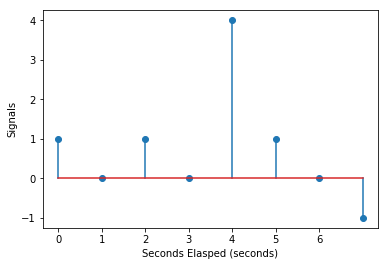
\includegraphics[scale=0.6]{../c1.png}
    \caption{$\operatorname{corr}_{\vec{r}_1}(\vec{s})$}
\end{figure}

\begin{figure}[H]
    \centering
    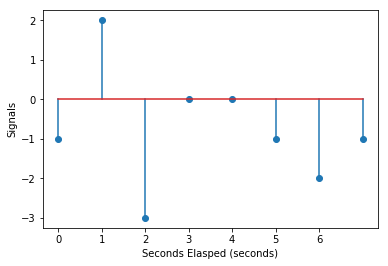
\includegraphics[scale=0.6]{../c2.png}
    \caption{$\operatorname{corr}_{\vec{r}_2}(\vec{s})$}
\end{figure}

\begin{figure}[H]
    \centering
    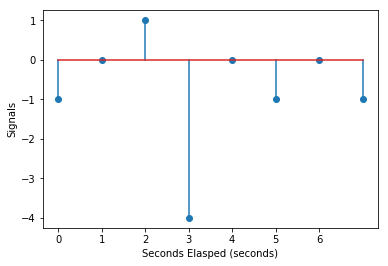
\includegraphics[scale=0.6]{../c3.png}
    \caption{$\operatorname{corr}_{\vec{r}_3}(\vec{s})$}
\end{figure}
}


\item{Based on the cross-correlated signals, determine the delays (in seconds) for all 3 received signals $\vec{r}_1$, $\vec{r}_2$, and $\vec{r}_3$.}

\note{Remind the students that the index in \textbf{Seconds Elapsed} corresponding to the maximum correlation is the same as the delays in seconds elapsed.}

\sol{Observing the plots for all 3 signals, we can see that the first received signal has a delay of 4 seconds, the second received signal has a delay of 1 second, and the last received signal has a delay of 2 seconds.
}

\item{Given that the radio signal has a transmission speed of $v$, and assume all delays are relative to the source signal $\vec{s}$ (this means we assume $\vec{s}$ is received at time $t = 0$), find the distance $d_1$, $d_2$, and $d_3$ between the user location and the 3 satellites in orbit.}

\note{For this part, it is helpful to give the students a more intuitive explanation that the delay of the received signal corresponds to the time it takes for the signal to reach the user.}

\sol{
Using the distance formula:
$$d = v \cdot \tau,$$
where $v$ is the transmission speed, $\tau$ is the delay (in seconds).
we can find the distances between the user location and the satellites to be:
$$d_1 = 4v, \;\; d_2 = v, \;\; d_3= 2v.$$
}
\end{enumerate}